\chapter{Additional Problems}

\section{Renting One Floor Out}

The second floor will combine four different departments to allow for space in the first floor. The new layout can be seen in figure \ref{fig:2nd_floor_varient}.
\begin{figure}[!h]
    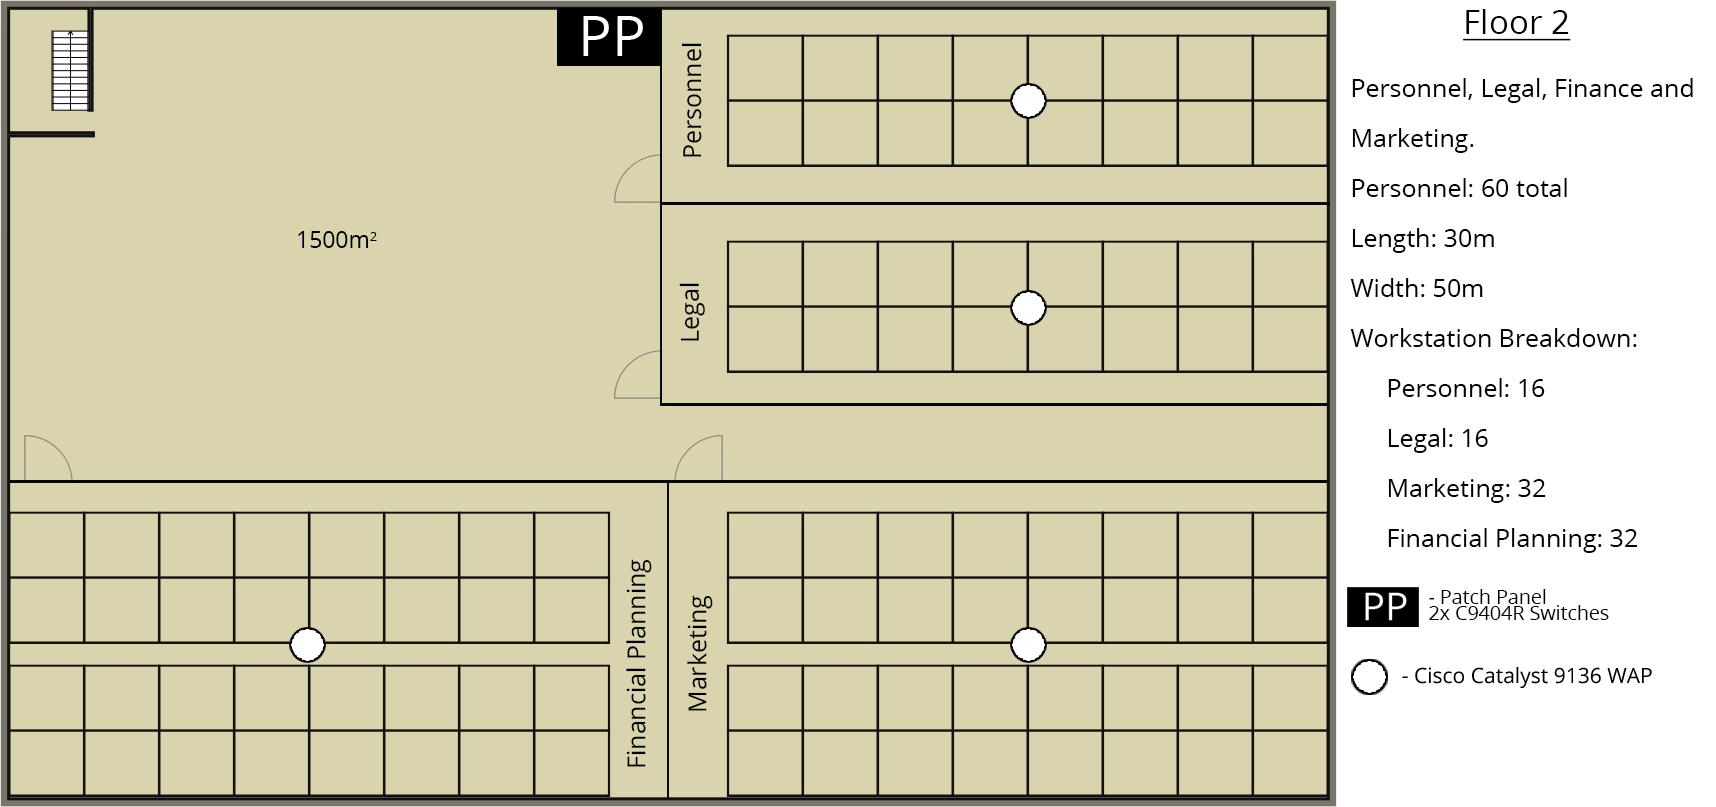
\includegraphics[width=15cm]{Figures/2nd-Floor-Varient.png}
    \caption{2nd floor plan combining 4 different departments}
    \label{fig:2nd_floor_varient}
\end{figure}

\begin{figure}[h]
    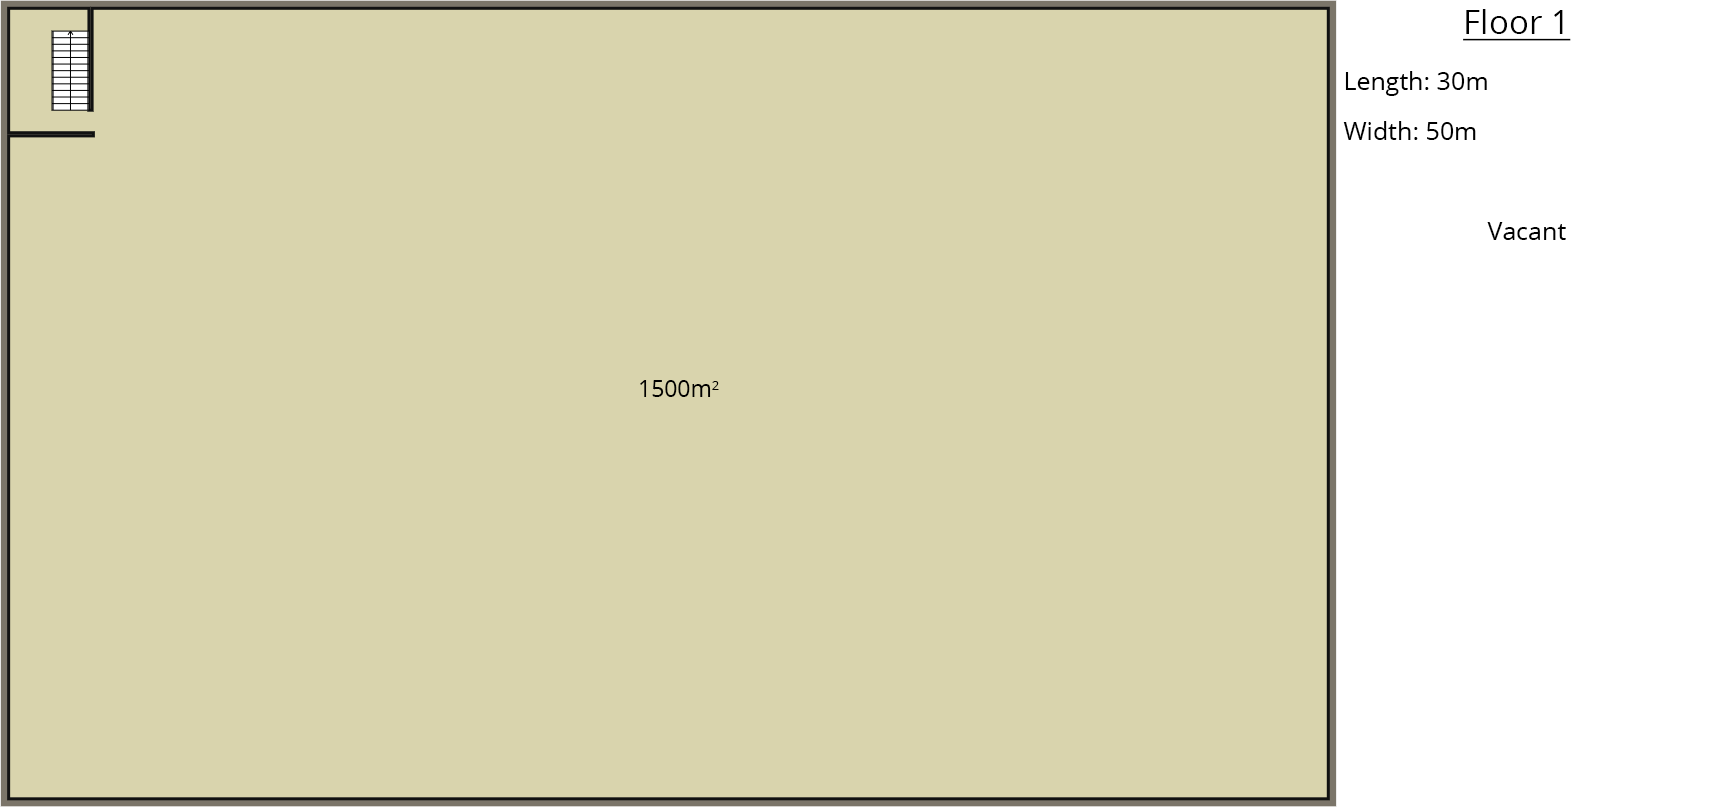
\includegraphics[width=15cm]{Figures/1st-Floor-varient.png}
    \caption{1st floor vacant plan}
    \label{fig:1st_floor_empty}
\end{figure}

The design and addressing specifications sections 4 and 5 are able to be reconfigured to place the occupants of floor 1 (currently financial planning and legal and accounting) and place them physically and logically on floor 2. This would include them being on the floor 2 subnet and no longer connected to floor 1. This vacant floor is then available for renting and is segregated on its own network.

\section{Splitting Between Two Buildings}
The servers that are able to give access to VPN and email are located within the DMZ, these will be accessible from the old HQ building network if Yotsuba decide to use it. The addressing scheme also allows the possiblity of adding many more devices to the internal network structure, so if they were to run the cabling between the buildings it could be incorporated directly. 
Running Single mode fiber between buildings.
